\documentclass[
	12pt,				% tamanho da fonte
	oneside,			% para impressão em recto e verso. Oposto a oneside
	a4paper,			% tamanho do papel. 
	english,			% idioma adicional para hifenização
	brazil,				% o último idioma é o principal do documento
	]{abntex2}

% ---
% Pacotes fundamentais 
% ---
\usepackage{lmodern}			% Usa a fonte Latin Modern
\usepackage[T1]{fontenc}		% Selecao de codigos de fonte.
\usepackage[utf8]{inputenc}		% Codificacao do documento (conversão automática dos acentos)
\usepackage{indentfirst}		% Indenta o primeiro parágrafo de cada seção.
\usepackage{color}				% Controle das cores
\usepackage{graphicx}			% Inclusão de gráficos
\usepackage{microtype} 			% para melhorias de justificação
\usepackage{multicol}
\usepackage{multirow}
\usepackage[brazilian,hyperpageref]{backref}	 % Paginas com as citações na bibl
\usepackage[alf]{abntex2cite}	% Citações padrão ABNT
\usepackage{listings}
\usepackage{float}

\lstset{
  showspaces=false,
  showtabs=false,
  breaklines=true,
  showstringspaces=false,
  breakatwhitespace=true,
  commentstyle=\color{green},
  keywordstyle=\color{blue},
  stringstyle=\color{red},
  basicstyle=\ttfamily
}

% --- 
% CONFIGURAÇÕES DE PACOTES
% --- 

% ---
% Configurações do pacote backref
% Usado sem a opção hyperpageref de backref
\renewcommand{\backrefpagesname}{Citado na(s) página(s):~}
% Texto padrão antes do número das páginas
\renewcommand{\backref}{}
% Define os textos da citação
\renewcommand*{\backrefalt}[4]{
	\ifcase #1 %
		Nenhuma citação no texto.%
	\or
		Citado na página #2.%
	\else
		Citado #1 vezes nas páginas #2.%
	\fi}%
% ---

% ---
% Informações de dados para CAPA e FOLHA DE ROSTO
% ---
\titulo{Prática 5: Jantar dos Filsósofos(Threads)}
\autor{Pedro Inácio Rodrigues Pontes}
\local{Belo Horizonte, Brasil}
\data{2025}
\instituicao{%
  Universidade Federal de Minas Gerais
  \par
  Colégio Técnico
  \par
  Curso Técnico em Desenvolvimento de Sistemas}

\definecolor{blue}{RGB}{41,5,195}

\makeatletter
\hypersetup{
     	%pagebackref=true,
		pdftitle={\@title}, 
		pdfauthor={\@author},
    	pdfsubject={\imprimirpreambulo},
		colorlinks=true,       		% false: boxed links; true: colored links
    	linkcolor=blue,          	% color of internal links
    	citecolor=blue,        		% color of links to bibliography
    	filecolor=magenta,      		% color of file links
		urlcolor=blue,
		bookmarksdepth=4
}
\makeatother

\renewcommand{\thesection}{\arabic{section}}
\setlength{\parindent}{1.3cm}
\setlength{\parskip}{0.2cm} 

\makeindex


\begin{document}

\selectlanguage{brazil}
\frenchspacing 

\imprimircapa

{
\ABNTEXchapterfont

\textual

% ----------------------------------------------------------
% Introdução (exemplo de capítulo sem numeração, mas presente no Sumário)
% ----------------------------------------------------------
\section{Introdução}

O objetivo da presente prática foi a implementação do Jantar dos Filósofos, tendo em vista o aprendizado do gerenciamento de recursos compartilhados em um ambiente concorrente.

Tal situação consiste em, de acordo com o enunciado da prática, "Imagine cinco filósofos sentados em torno de uma mesa circular, com um prato de comida em frente a cada um. Entre cada par de pratos, há um garfo. Os filósofos passam o tempo pensando e, ocasionalmente, tentam comer. Para comer, um filósofo precisa ter acesso a dois garfos: o garfo à sua esquerda e o garfo à sua direita. Se um filósofo não conseguir obter os dois garfos, ele não pode comer e deve continuar pensando."

\section{Desenvolvimento}

Para estruturar a implementação dos resultados, foram criadas as classes Program, Philosopher e Console Lock.

Program é a main, gerenciando o programa e a atuação de suas classes. Philosopher implementa os filósofos e suas lógicas, com destaque à de gerenciamento de recursos. ConsoleLock é uma classe simples para as Threads escreverem no console, já implementando o Lock para evitar conflitos entre elas (race conditions).

A seguuir temos um detalhamento das partes mais significativas de Philospher e Program.

\subsection{Philosopher}

Pode se definir o comportamento inicial básico da classe vendo seu construtor:

\begin{lstlisting}
public Philosopher(string name, string thought, SemaphoreSlim[] forks)
{
    Name = name;
    Thought = thought;
    Id = Interlocked.Increment(ref _nextId);
    Forks = forks;
}
\end{lstlisting}

A lógica do filósofo é representada em Live():

\begin{lstlisting}
public void Live()
{
    Think();
    Eat();
}
\end{lstlisting}

Em Think ele simplesmente emite o pensamento definido em seu construtor, antecedido por sua identificação pelo nome.

Em Eat primeiramente é chamado o método GetFork, que consite no método para o filósofo obter os garfos, que são gerenciados a partir do SemaphoreSlim, assim é chamado um Wait para os garfos que corresponde à esquerda e direita dele (calculadas a partir do seu id). É feita também uma lógica para implementar um lógica fixa de obtenção dos garfos (menor para o maior), evitando o um ciclo de espera circular que caracteriza o deadlock. Este fenômeno seria causado quando todos os filósofos tentarem pegar os garfos ao mesmo tempo, e o filósofo 5 tentaria pegar o garfo 5 antes do 1, o que ocorre seguindo a lógica normal de obtenção, e com isso, o filósofo 4 não conseguiria pegar o seu segundo garfo, que já estaria sendo usado pelo 5, e o 5 não conseguiria pegar seu segundo também, que já estaria sendo usado pelo 1. Com a implementação desse ordenamento não ocorre tal ciclo, pois o filósofo 5 primeiro tenta pegar o garfo 1 e depois o 5.

Após o GetFork o filosófo emite uma mensagem demonstrado que está comendo e, por fim, libera esses garfos a partir de ReleaseFork, que chama o método Release do SemaphoreSlim nos garfos utilizados.

Segue o método principal de gerenciamento de recursos GetFork:

\begin{lstlisting}
public void GetFork()
{
    var leftFork = getLeftFork();
    var rightFork = getRightFork();
    if (leftFork > rightFork)
    {
        var temp = leftFork;
        leftFork = rightFork;
        rightFork = temp;
    }
    Forks[leftFork].Wait();
    Forks[rightFork].Wait();
}
\end{lstlisting}

A classe também possui um método Start, que gera uma Task que roda infinitamente o ciclo Live(), que está dentro de um While(true)

\subsection{Program}

Cria e inicializa o Array de Filósofos e o dos garfos SemaphoreSlim. Segue seu cerne:

\begin{lstlisting}
for(int i = 0; i < 5; i ++)
{
    forks[i] = new SemaphoreSlim(1, 1); 
}
for (int i = 0; i < philosophers.Length; i++)
{
    philosophers[i] = new Philosopher(names[i], thoughts[i], forks);
    philosophers[i].Start();
}
\end{lstlisting}

\section{Resultados}

\begin{figure}[H]
    \centering
    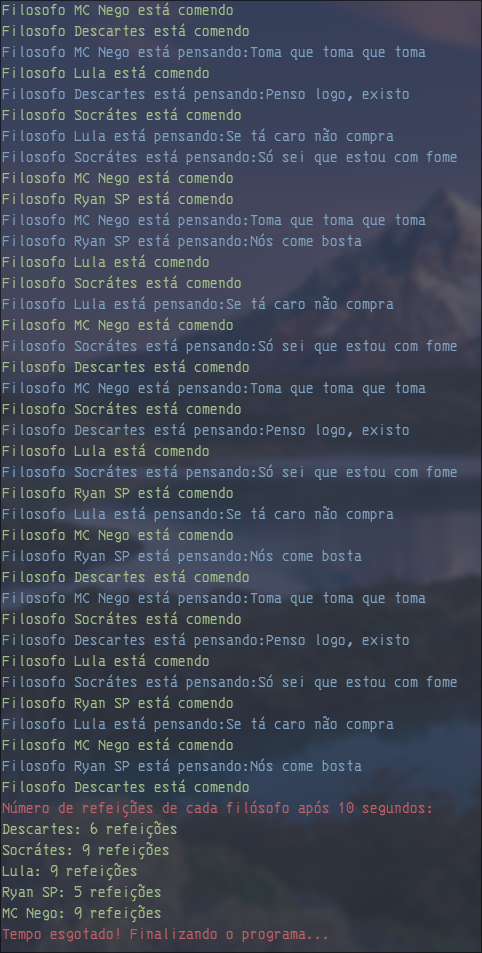
\includegraphics[width=0.7\textwidth]{img1.png}
    \caption{Filósofos emitindo seus pensamentos e comendo, com um log final de quantas vezes cada um comeu em 10 segundos de execução}
    \label{fig:img1}
\end{figure}
\section{Conclusão}

Todos os resultados foram alcançados, sendo evitados os deadlocks e a starvation. O método da ordem fixa de obtenção dos garfos foi o melhor para o contexto, pois sua altenativa seria um método tentativa com falha, o qual pode vir a gerar starvation se não implementado adequadamente, pois um filósofo pode conseguir os dois garfos constantemente, evitando que outros consigam os dois garfos e causando deles sempre abandonarem a tentativa em que estavam de comer por falha. Isso seria evitado implementando uma fila ou política de acesso aos garfos, mas deixaria o programa mais complexo que com o método da ordem fixa, além de pior em relação a desempenho pelos filósofos poderem abandonar suas tentativas se os dois garfos não estiverem disponíveis no momento exato em que o método para comer for iniciado.

\end{document}
